%% Requires compilation with XeLaTeX or LuaLaTeX
\documentclass[aspectratio=169,10pt,xcolor={table,dvipsnames},t]{beamer}
\usetheme{UCBerkeley}
\hypersetup{colorlinks=true, linkcolor=blue, citecolor=blue, urlcolor=blue}
\usepackage{xcolor}

\title[lecture 06]{Next Generation Data Centers and Energy Management Systems}
\subtitle{Lecture 6A:Chip Cooling: Heat Conduction and Thermal Interface Materials}
% Radiation heat transfer for Lecture XX??? Can be done in Spacecraft Thermal Control
\author{Prof. Thomas M. Schutzius}
\institute{Department of Mechanical Engineering}
\date{Fall 2026}

\begin{document}

\begin{frame}
  \titlepage
\end{frame}

% Uncomment these lines for an automatically generated outline.
%\begin{frame}{Outline}
%  \tableofcontents
%\end{frame}

{
\smallframetitle % small frame title
\setbeamertemplate{background}{} % Hides background for this frame
\setbeamertemplate{footline}{}   % Reclaims the bottom space

% Learning plan. Highlight in bold the item we are covering in this lecture.
\begin{frame}
	\frametitle{Learning Plan}
	\begin{itemize}
		\item Introduction to Data Center Systems and Thermodynamics 
		\item Psychrometrics and Heat Transfer
		\item Performance Metrics and Standards
		\item Applied Computational Fluid Dynamics (CFD)
		\item Liquid Cooling \& Advanced Heat Transfer
		\item \textbf{Chip Cooling: Heat Conduction and Thermal Interface Materials}
		\item Power Delivery and Infrastructure (Energy sources: Geothermal, Solar, Nuclear, etc.)
		\item Overview of Simulation Field; the Concept of a Digital Twin 
		\item Machine Learning and Optimization Tools 
		\item Modeling and Simulation of an Energy Management System 
		\item Control Systems and Optimization 
		\item Spacecraft Thermal Control
		\item Final Project Work, Peer Feedback, and Mentor Check-in 
		\item Symposium 
	\end{itemize}		
\end{frame}

% Learning objectives go here.
\begin{frame}
	\frametitle{Learning Objectives} 
		\begin{itemize}
			\item Understand the thermodynamic limits of computing (Landauer's Principle).
			\item Analyze modern chip architectures and their thermal implications.
			\item Model heat conduction through a multi-layer chip cooling stack.
		\end{itemize}		
\end{frame}


% Include the typical layout of a data center facility in each lecture.
\begin{frame}
	\frametitle{Typical layout of a data center facility}
		\begin{figure}
			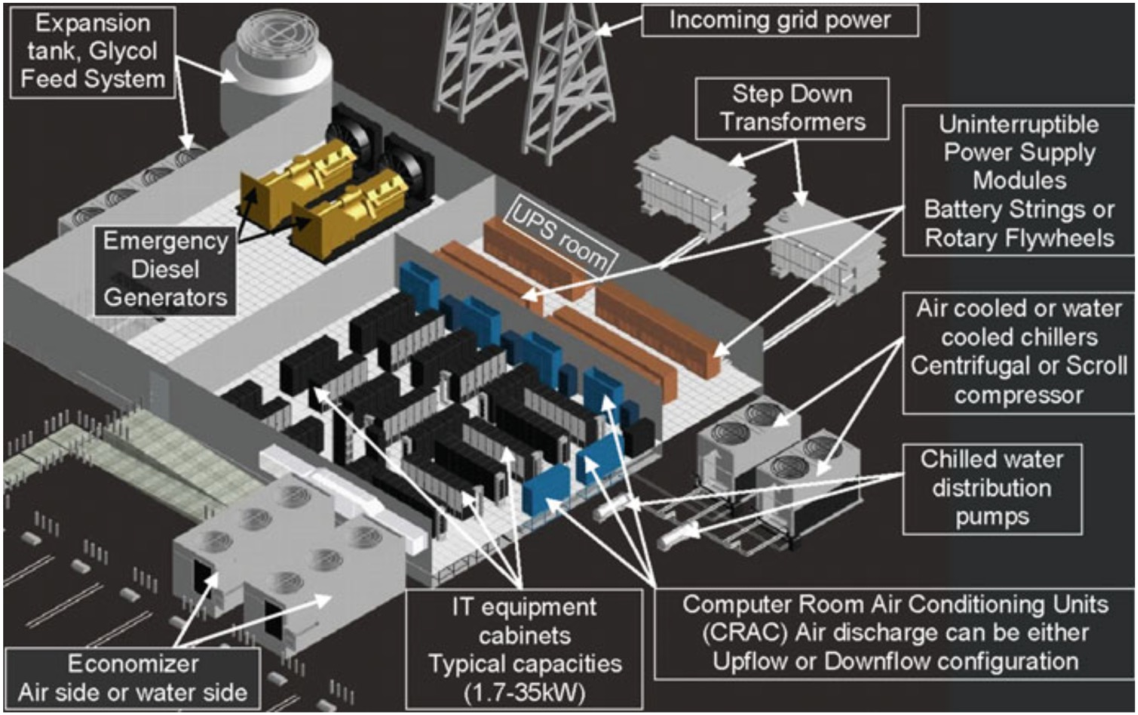
\includegraphics[width=0.65\textwidth]{../figures/joshi2021introduction-figure-01-01.pdf}
%			\vspace{-0.5cm }
		 \caption{(Figure 1.1 in Ref. \cite{joshi2012energy}).}
		\end{figure}
\end{frame}

\begin{frame}
	\frametitle{Project 1: Feedback} 
		\begin{itemize}
			\item Check that you have addressed every task listed in the project tasks section of the description before submitting.
			\item Use the template. Its purpose is to simplify your lives. You don't need to add sections, modify the text size, etc.
			\item Ben: Come to office hours or send me questions via email.
		\end{itemize}		
\end{frame}

% If there is an upcoming seminar, please include here
\begin{frame}{Thermodynamics of Computing}
    \begin{itemize}
        \item \textbf{Why is heat generated?} Irreversible computing operations (e.g., erasing a bit) increase entropy.
        \item \textbf{Landauer's Principle:} The minimum energy required to erase one bit of information is $E_{min} = k_B T \ln 2$.
        \item \textbf{Metric:} Joules per FLOP (or bit flip).
        \item \textbf{Modern vs. Limit:} Modern systems are orders of magnitude away from the thermodynamic limit.
    \end{itemize}
    \begin{figure}
        \centering
        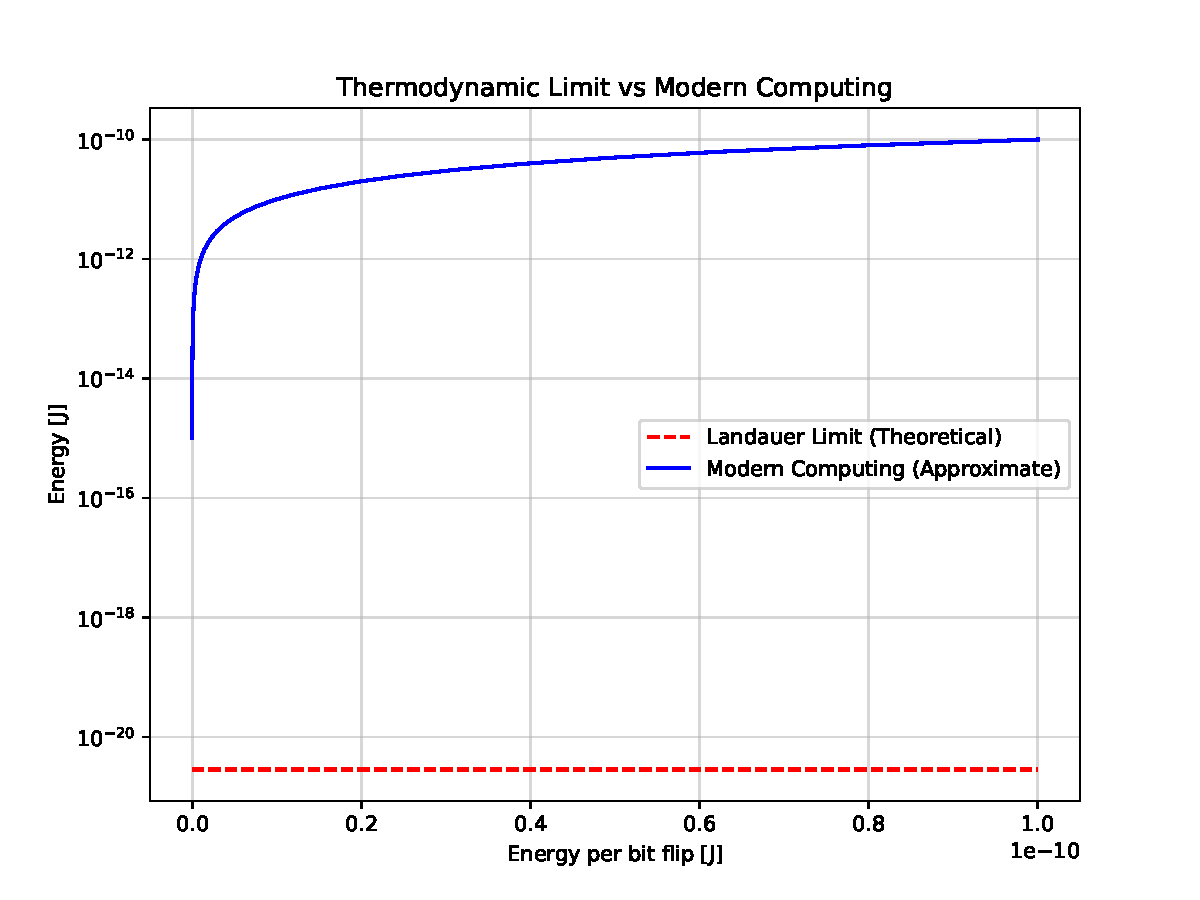
\includegraphics[width=0.5\textwidth]{../figures/thermodynamics_limit.pdf}
        \caption{Comparison of energy per bit flip: Modern vs. Landauer Limit.}
    \end{figure}
\end{frame}

    \begin{frame}
        \frametitle{\href{https://datahub.berkeley.edu/user-redirect/git-pull?repo=https://github.com/mtsn-lab/me137-237a&subPath=examples/thermodynamicsOfComputing.ipynb}{Thermodynamics of Computing Notebook}}
            \begin{figure}
                \centering
                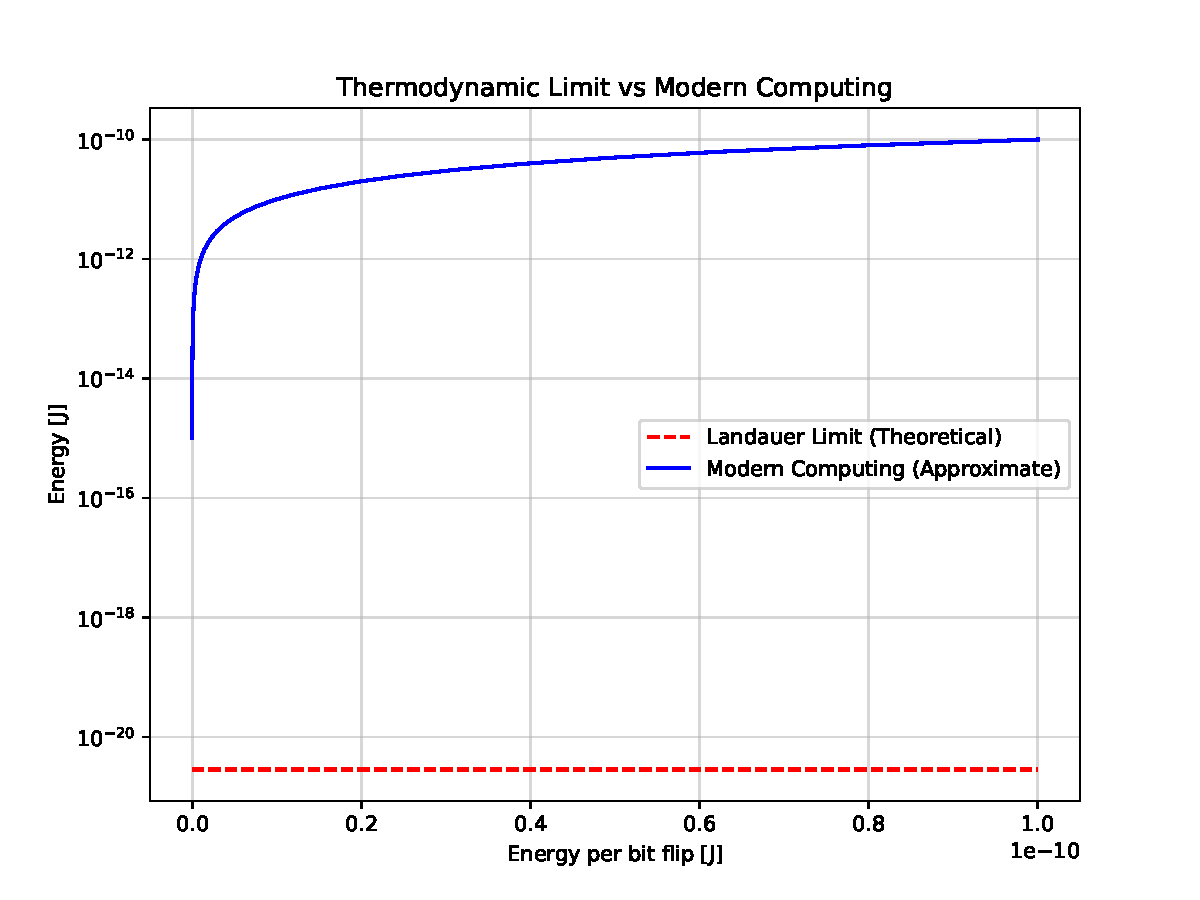
\includegraphics[width=0.4\textwidth]{../figures/thermodynamics_limit.pdf}
                 \caption{Energy scales in computing.}
            \end{figure}
    \end{frame}

\begin{frame}{Modern Chip Architecture}
    \begin{itemize}
        \item \textbf{Components:}
            \begin{itemize}
                \item Logic Die (CPU/GPU cores)
                \item Memory (HBM - High Bandwidth Memory)
                \item Interposer (Silicon or organic substrate connecting die and memory)
                \item Vias (TSVs - Through-Silicon Vias)
            \end{itemize}
        \item \textbf{Heat Generation:} Concentrated in the logic die (high power density).
        \item \textbf{Thermal Management Stack:}
            \begin{itemize}
                \item Thermal Interface Material (TIM)
                \item Heat Spreader (Integrated Heat Spreader - IHS)
                \item Vapor Chamber (Phase change cooling)
                \item Heat Sink (Convection to air/liquid)
            \end{itemize}
    \end{itemize}
\end{frame}

\begin{frame}{Heat Transfer Modeling}
    \begin{itemize}
        \item \textbf{Physics:} 1D Steady-state heat conduction with heat generation $\dot{q}$:
        $$\frac{d}{dx}\left(k \frac{dT}{dx}\right) + \dot{q} = 0$$
        \item \textbf{Application:} Modeling the temperature gradient across the cooling stack:
        $$\text{Silicon} \to \text{TIM} \to \text{Spreader} \to \text{Vapor Chamber} \to \text{Heat Sink}$$
    \end{itemize}
    \begin{figure}
        \centering
        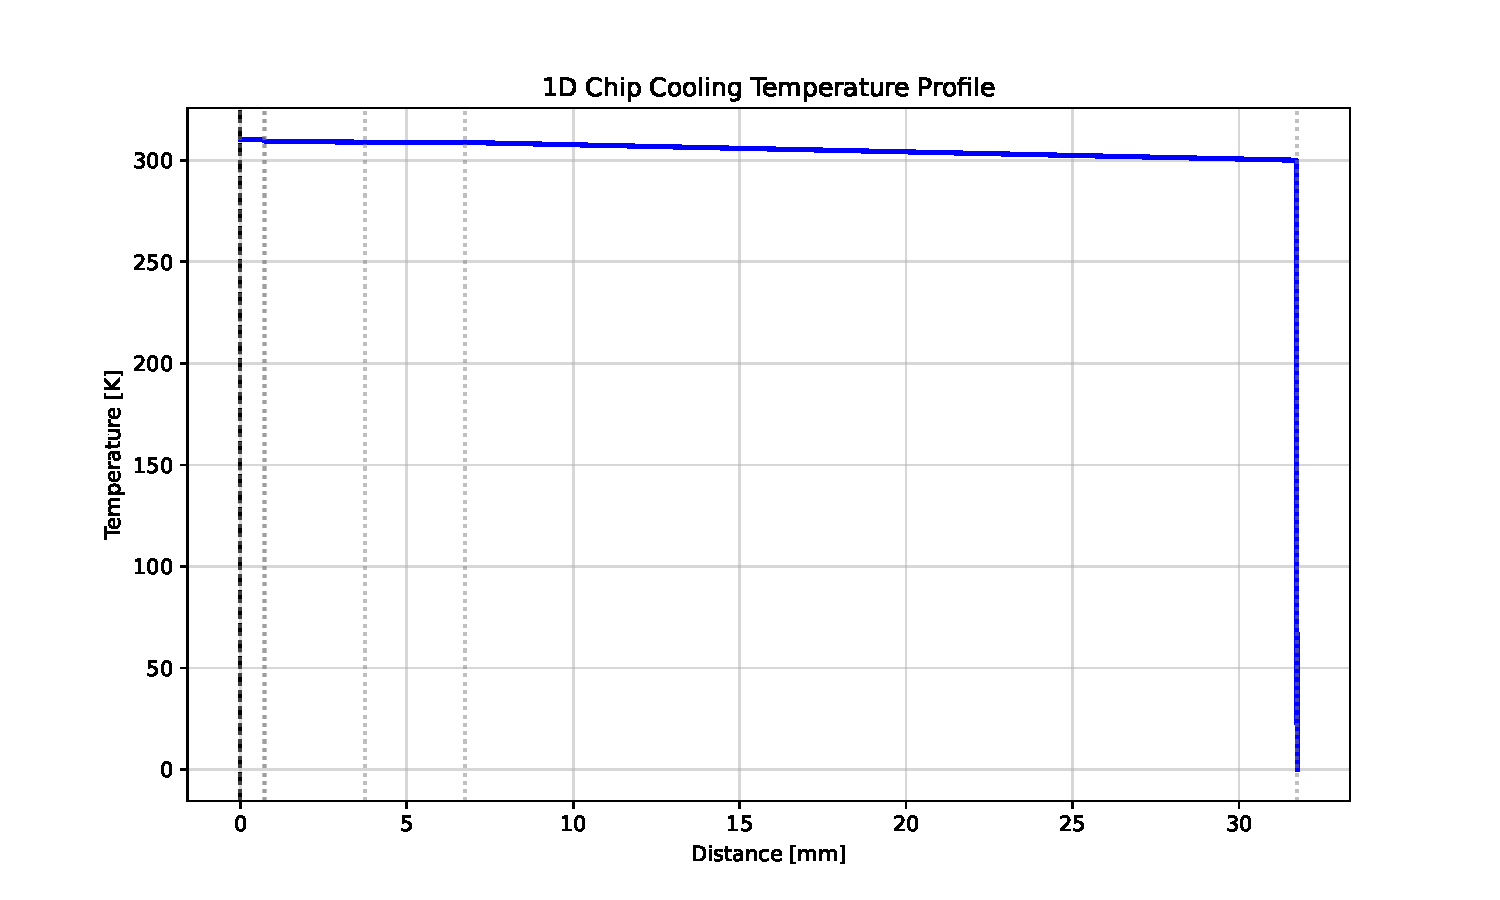
\includegraphics[width=0.6\textwidth]{../figures/chip_temperature_profile.pdf}
        \caption{Predicted temperature profile across the cooling stack.}
    \end{figure}
\end{frame}

\begin{frame}
	\frametitle{\href{https://datahub.berkeley.edu/user-redirect/git-pull?repo=https://github.com/mtsn-lab/me137-237a&subPath=examples/chipHeatTransfer.ipynb}{Chip Heat Transfer Notebook}}
		\begin{figure}
			\centering
			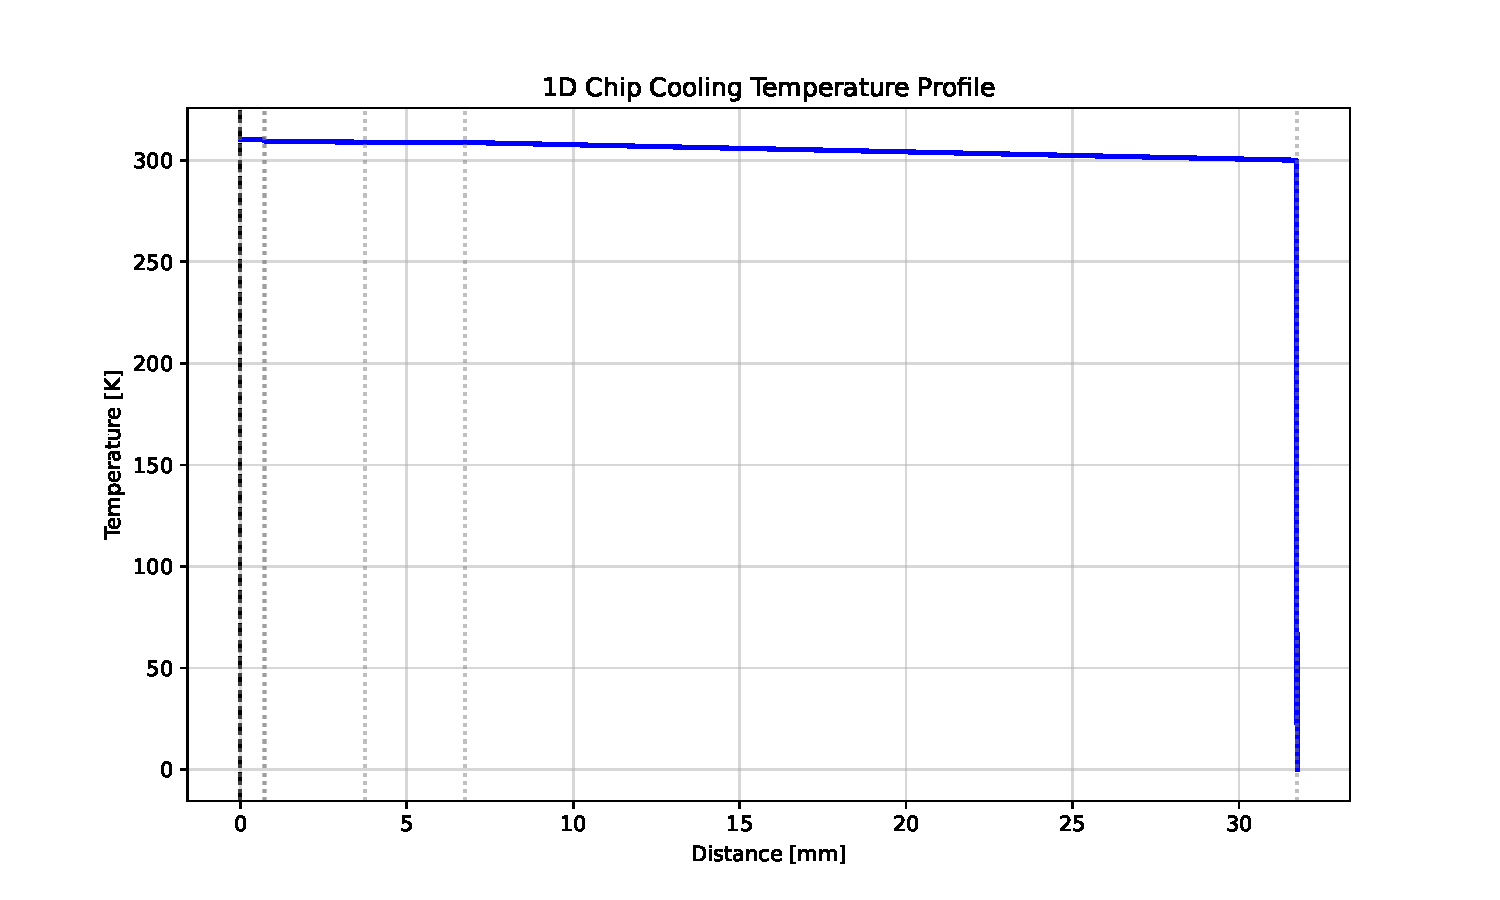
\includegraphics[width=0.4\textwidth]{../figures/chip_temperature_profile.pdf}
		 \caption{Thermal profile simulation.}
		\end{figure}
\end{frame}

\begin{frame}
	\frametitle{Seminar 3}
		\begin{itemize}
			\item Name
			\item Title: TBD
			\item Date: TBD
			\item Time: 15:30 (Berkeley Time)
			\item Location: GSPP 150
		\end{itemize}
\end{frame}


}
% ------------------------------------------------------------------------------------------------------------------------------------------------------------------------------------
% This is an example for how I link the Jupyter notebook example to the slide I am showing.
% If there is a figure output from the Jupyter notebook, that should be shown here. The Jupyter notebook should be located in me137-237a/examples
% The figure output from the Jupyter notebook should go in the directory me137-237a/lectures/figures

%\begin{frame}
%	\frametitle{\href{https://datahub.berkeley.edu/user-redirect/git-pull?repo=https://github.com/mtsn-lab/me137-237a&subPath=examples/fanLaws.ipynb}{Fan Laws}}
%		\begin{figure}
%			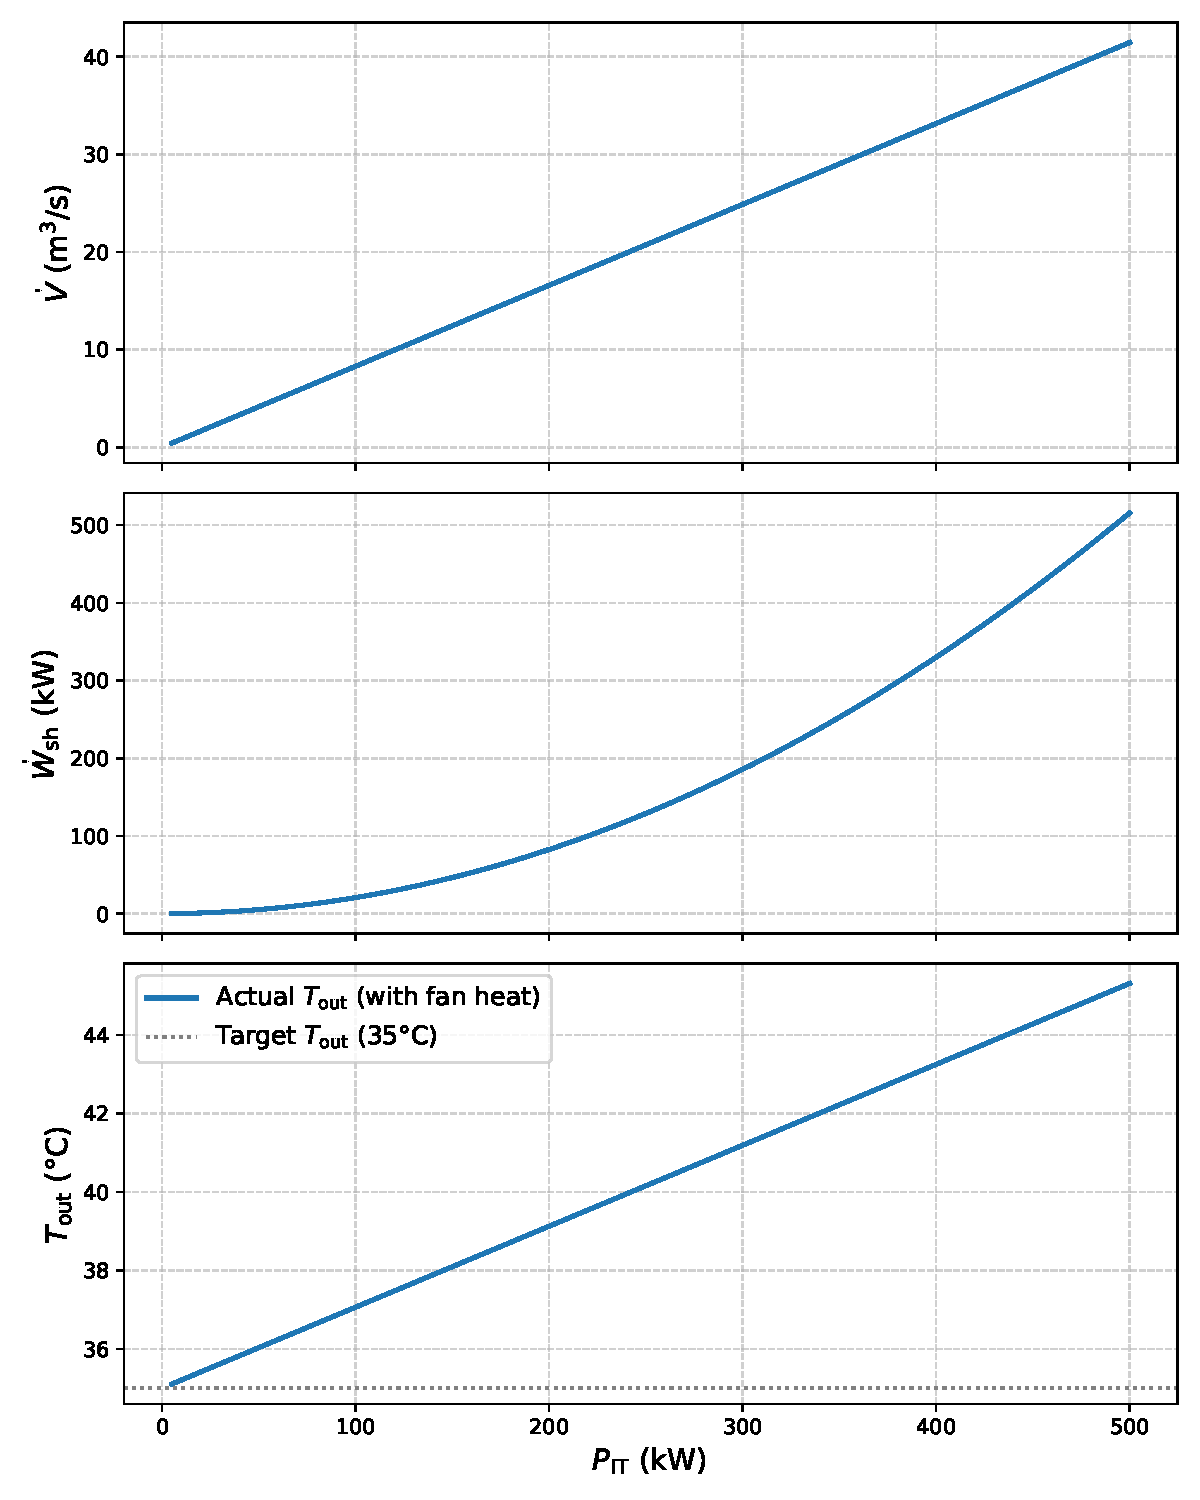
\includegraphics[width=0.4\textwidth]{../figures/rack_cooling_plots.pdf}
%		 \caption{Solution to the Pohlhausen equation. Read his biography \href{https://doi.org/10.1146/annurev.fl.16.010184.000245}{here}.}
%		\end{figure}
%\end{frame}
% ------------------------------------------------------------------------------------------------------------------------------------------------------------------------------------


{
\setbeamertemplate{bibliography item}[text] % Replaces default icons with numbers
	\begin{frame}[allowframebreaks]{References}
		\bibliographystyle{plain}
		\bibliography{../../bibliography}
	\end{frame}
}

\end{document}
